\chapter{QUADRO TEÓRICO}

\par Utilizando o comando \texttt{\textbackslash par} para indicar o início de um parágrafo.
\par Outro parágrafo, agora modificando o tipo da fonte: \texttt{void calcular(int x)}.

\section{Recursos}

\par Exemplo de parágrafo utilizando comando para formatar em itálico as palavras em inglês, como por exemplo: \textit{pets, animals and software} e um exemplo de texto em negrigo: \textbf{grafo}.

\par Um tipo de citação: segundo \citeonline{correa2003plantas} as plantas \ldots.

\par Outro tipo de citação: as plantas \ldots \cite{correa2003plantas}.

\par Outro tipo de citação com página: \cite[p. 13]{correa2003plantas}.
\par Outro tipo ainda de citação com página:  \citeonline[p. 13]{correa2003plantas}.

\par Para referenciar seções e capítulos, é necessário colocar o \textbackslash label e a referência assim: na \autoref{sec:materiais} e no \autoref{cap:quadroMetodologico} são encontradas as informações\ldots

\par Exemplo de equação:

\begin{equation}
 \Delta Q = 
 \left[
 \frac{\sum_{in} + k_{i,in}}{2m} - 
 \left(
 \frac{\sum_{tot} + k_i}{2m}
 \right)^2
 \right] -
 \left[
 \frac{\sum_{in}}{2m} - 
 \left(\frac{\sum_{tot}}{2m}
 \right)^2 - 
 \left(\frac{k_i}{2m}
 \right)^2
 \right]
\end{equation}


\par Símbolos matemáticos só funcionam dentro do ambiente \texttt{equation} ou entre dois símbolos \$. Ex: Adiciona cada vértice $w \in N_d(v) \Delta \Gamma$ na região, os quais foram vistos por pelo menos a uma fração $\gamma$ dos vértices em $N_d(v)$.

\par Outra fórmula: $y=x^2$

\section{Materiais}
\label{sec:materiais}

\par Este parágrafo mostra um exemplo de um teste de nota de rodapé, utilizando o texto do documento da Univas\footnote{O nome “Desenvolvimento” é muito vago, portanto, não o utilize; prefira, de acordo com a situação, ``Fundamentação teórica'', ``Análise dos dados'', ``Objetivos'', ``Metodologia'', etc. }. Outro tipo de nota de rodapé\footnote{\cite{correa2003plantas}}.  Outro tipo ainda de nota de rodapé\footnote{\citeonline{correa2003plantas}}


\par Um exemplo de tabela é mostrado na Tabela~\ref{tab:informativa}


\begin{table} [h]
  \caption[Informação nutricioal dos alimentos]
          {Informação nutricioal dos alimentos \textbf{Fonte:} \cite{correa2003plantas}}
  \centering
  \begin{tabular}{|p{0.7in}|p{2in}|p{3in}|}
    \hline 
    \multicolumn{1}{|c|}{\textbf{Hortaliça}} & \multicolumn{1}{c|}{\textbf{Valor Nutricional}} & \multicolumn{1}{c|}{\textbf{Propriedades medicinais}} \\
    \hline 
Tomate
&Vitamina A, C, E e ferro, potássio
&Maior resistência aos vasos sanguíneos, combate a infecções\\
    \hline 
Cenoura
&Vitamina A, vitaminas do complexo B, cálcio, fósforo
&Regula o aparelho digestivo, purifica a bile e fortalece a pele\\
    \hline
Cebolinha
&Cálcio, ferro, niacina
&Estimula o apetite, ajuda na formação de ossos e dentes\\

    \hline
Alface
&Ferro, cálcio, niacina, vita\-mina C
&Combate insônia, ajuda na cicatrização dos tecidos\\

    \hline
Rúcula
&Iodo, vitaminas A e C
&Combate a fadiga, depura o sangue\\

    \hline
Erva cidreira
&Sais minerais
&Tonico nervoso, combate cólicas intestinais\\

    \hline 
  \end{tabular}
  \legend{Fonte: \cite{correa2003plantas}}
  \label{tab:informativa}
\end{table}

\par A seguir segue exemplo de listagem numérica:

\begin{enumerate}
  \item conteúdo do item 1;
  \item conteúdo do item 2;
  \item conteúdo do item 3;
  \item conteúdo do item 4;
  \item conteúdo do item 5;
  \item conteúdo do item 6;
  \item etc.
\end{enumerate}

\par Também é possível fazer a lista de itens:

\begin{itemize}
  \item conteúdo do primeiro item;
  \item conteúdo do segundo item;
  \item conteúdo do terceiro item;
  \item conteúdo do quarto item;
  \item conteúdo do quinto item;
  \item etc.
\end{itemize}

\par Um exemplo de imagem é mostrado na Figura~\ref{fig:exemplo1}.

\begin{figure}[h!]
  \centerline{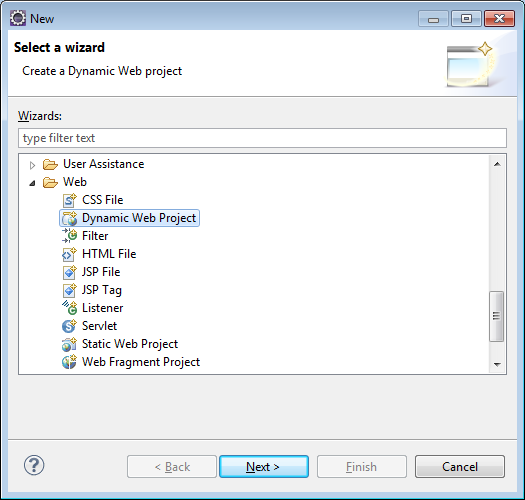
\includegraphics[scale=0.65]{./imagens/apendice_img1.png}}
  \caption[Exemplo de criação de um projeto Web no Eclipse]
          {Exemplo de criação de um projeto Web no Eclipse. \textbf{Fonte:} \cite{correa2003plantas}}
\label{fig:exemplo1}
\end{figure}

\par Perceba que o \LaTeX~faz a numeração automática das figuras e já adiciona na lista de figuras.

\par Agora a mesma imagem foi incluída, porém em escala menhor, conforme ilustra a Figura~\ref{fig:exemplo2}.:

\begin{figure}[h!]
  \centerline{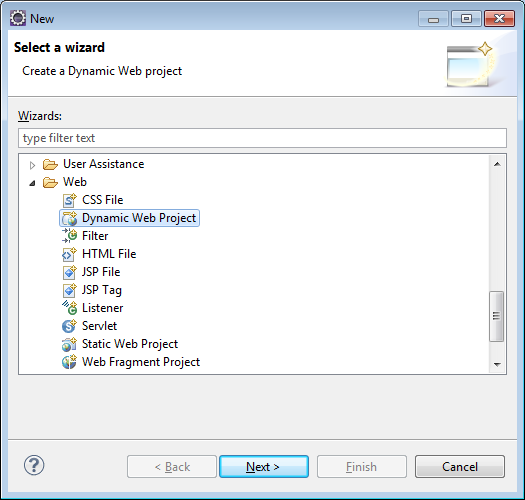
\includegraphics[scale=0.25]{./imagens/apendice_img1.png}}
  \caption[Mesma imagem em escala menor]
          {Mesma imagem em escala menor. \textbf{Fonte:} \cite{correa2003plantas}}
\label{fig:exemplo2}
\end{figure}